\documentclass{article}
\usepackage{cmap}
\usepackage[utf8]{inputenc}
\usepackage[english,ukrainian]{babel}
\usepackage{graphicx}
\usepackage{geometry}
\usepackage{listings}
\usepackage{indentfirst}
\usepackage{subfigure}
\usepackage{caption}
\usepackage{amsmath}
\geometry{
	a4paper,
	left=20mm,
	right=20mm,
	top=20mm,
	bottom=20mm
}
\lstset{
	extendedchars=\true,
	tabsize=4,
	language=python,
	showstringspaces=false,
	showtabs=false,
	frame=lrtb,
	columns=fixed,
	keepspaces,
	breaklines=true
}
\graphicspath{ {pictures} }
\setlength{\parindent}{4em}
\newcommand\subject{Чисельні методи ПЗ}
\newcommand\lecturer{доцент кафедри ПЗ\\Мельник Н.Б.}
\newcommand\teacher{асистент кафедри ПЗ\\Гарматій Г.Ю.}
\newcommand\mygroup{ПЗ-16}
\newcommand\lab{3}
\newcommand\theme{Розв’язування систем лінійних алгебраїчних рівнянь методом Крамера та методом оберненої матриці}
\newcommand\purpose{Ознайомлення на практиці з методом Крамера та методом
	оберненої матриці розв’язування систем лінійних алгебраїчних рівнянь}

\begin{document}
	\begin{large}
		\begin{titlepage}
			\thispagestyle{empty}
			\begin{center}
				\textbf{МІНІСТЕРСТВО ОСВІТИ І НАУКИ УКРАЇНИ\\
					НАЦІОНАЛЬНИЙ УНІВЕРСИТЕТ "ЛЬВІВСЬКА ПОЛІТЕХНІКА"}
			\end{center}
			\begin{flushright}
				Інститут \textbf{КНІТ}\\
				Кафедра \textbf{ПЗ}
			\end{flushright}
			\vspace{200pt}
			\begin{center}
				\textbf{ЗВІТ}\\
				\vspace{10pt}
				До лабораторної роботи № \lab\\
				\textbf{На тему}: “\textit{\theme}”\\
				\textbf{З дисципліни}: “\subject”
			\end{center}
			\vspace{90pt}
			\begin{flushright}
				
				\textbf{Лектор}:\\
				\lecturer\\
				\vspace{28pt}
				\textbf{Виконав}:\\
				
				студент групи \mygroup\\
				Коваленко Д.М.\\
				\vspace{28pt}
				\textbf{Прийняла}:\\
				
				\teacher\\
				
				\vspace{28pt}
				«\rule{1cm}{0.15mm}» \rule{1.5cm}{0.15mm} 2022 р.\\
				$\sum$ = \rule{1cm}{0.15mm}……………\\
				
			\end{flushright}
			\vspace{\fill}
			\begin{center}
				\textbf{Львів — 2022}
			\end{center}
		\end{titlepage}
		
		\begin{description}
			\item[Тема.] \theme.
			\item[Мета.] \purpose.
		\end{description}
		
		\section*{Теоретичні відомості}
		\subsection*{Метод оберненої матриці}
		Цей метод ґрунтується на обчисленні
		оберненої матриці $A^{-1}$ , яка існує лише при умові, коли визначник матриці $A$
		відмінний від нуля $\det{A}\ne0$.
		
		Для знаходження оберненої матриці $A^{-1}$ необхідно застосувати алгоритм,
		який складається з таких пунктів:
		\begin{enumerate}
			\item Обчислення визначника $\det{A}$ матриці $A$ коефіцієнтів системи . Якщо він
			не дорівнює нулеві, то продовжуємо розв’язувати систему лінійних алгебраїчних рівнянь. Якщо $\det{A}=0$,
			то матриця $A$ є виродженою і для неї не існує оберненої.
			\item Формування матриці $\overline{A}$, елементами якої є алгебраїчні доповнення
			матриці $A$.
			\item Транспонування матриці $\overline{A}^T$.
			\item Визначення оберненої матриці за формулою $\det{A}=\frac{\overline{A}}{\det{A}}$.
		\end{enumerate}
	
		\subsection*{Метод Крамера}
		Для знаходження невідомихix застосовують
		формули Крамера:
		\begin{gather}\nonumber
			x_i=\frac{\det{A_i}}{\det{A}}, \hspace{28pt}i=1,2,3...n, 
		\end{gather}
		де $\det{A}$ - визначник матриці $\det{A_i}$ - визначник матриціi $A$, яку отримують з
		матриці $A$ шляхом заміни її  $i$-го стовпця стовпцем вільних членів.

		\section*{Лабораторне завдання}
		\begin{enumerate}
			\item Ознайомитись з теоретичними відомостями.
			\item Скласти програму розв’язування системи лінійних алгебраїчних рівнянь
			методом оберненої матриці та методом Крамера.
			\begin{gather}\nonumber
				\left\{\begin{array}{@{}l@{}}
				0.34x_1 + 0.71x_2 + 0.63x_3 = 2.08\\\nonumber
				0.71x_1 - 0.65x_2 - 0.18x_3 = 0.17\\\nonumber
				1.17x_1 - 2.35x_2 + 0.75x_3 = 1.28\nonumber
				\end{array}\right.\,
			\end{gather}
		\end{enumerate}

		\section*{Хід роботи}
		\subsection*{Метод оберненої матриці}
		\begin{gather}\nonumber
			X=A^{-1}B\\\nonumber
				X=\begin{pmatrix}
					x_1\\
					x_2\\
					x_3\\
				\end{pmatrix}
				\hspace{28pt}
				A=\begin{pmatrix}
					0.34 & 0.71 & 0.63\\
					0.71 & 0.65 & 0.18\\
					1.17 & 2.35 & 0.75
				\end{pmatrix}
			\hspace{28pt}
			B=\begin{pmatrix}
				2.08\\
				0.17\\
				1.28
			\end{pmatrix}
		\end{gather}
	\begin{gather}
			\det(A)=\begin{vmatrix}\nonumber
				0.34 & 0.71 & 0.63\\
				0.71 & 0.65 & 0.18\\
				1.17 & 2.35 & 0.75
			\end{vmatrix} = 0.3654
		\\
			A_{11}=(-1)^{1+1}\begin{vmatrix}\nonumber
				0.65 & 0.18\\
				2.35 & 0.75
			\end{vmatrix} = 0.0645
			\\
			\overline{A}^T = \begin{pmatrix}\nonumber
				0.0645 & 0.948 & -0.2817\\
				-0.3219 & -0.4821 & 0.3861\\
				0.908 & 0.0317 & -0.2831
			\end{pmatrix}
			\\
			A^{-1} = \frac{1}{\det{A}}\overline{A}^T = \begin{pmatrix}\nonumber
				0.1765 & 2.5942 & -0.7635\\
				-0.8809 & -1.3193 & 1.0565\\
				2.4848 & 0.0867 & -0.7747
			\end{pmatrix}
			\\
			X=\begin{pmatrix}\nonumber
				0.1765 & 2.5942 & -0.7635\\
				-0.8809 & -1.3193 & 1.0565\\
				2.4848 & 0.0867 & -0.7747
			\end{pmatrix}
			\begin{pmatrix}\nonumber
				0.65 & 0.18\\
				2.35 & 0.75
			\end{pmatrix}
			=
			\begin{pmatrix}
				-0.1786\\
				-0.7041\\
				4.1915
			\end{pmatrix}
		\end{gather}
			
		\noindent\textit{\textbf{Код програми} (файл lab\_\lab1.py):}
		\begin{lstlisting}
import numpy as np

def data_to_matrix(path):
	return (
		np.loadtxt(open(path,"rb"), delimiter=",", usecols=[0,1,2]),
		np.loadtxt(open(path,"rb"), delimiter=",", usecols=3),
	)

def inverse_matrix_method(A, B, n):
	""" Метод оберненої матриці """
	print(inverse_matrix_method.__doc__)
	A_1 = np.array(A) # Обернена матриця коефіцієнтів
	for i in range(n):
		for j in range(n):
			tmp = np.delete(A, i, 0)
			tmp = np.delete(tmp, j, 1)
			A_1[i][j] = (-1)**((i) + (j)) * np.linalg.det(tmp) / np.linalg.det(A)
	A_1 = np.transpose(A_1)
	print(f"Обернена матриця: \n{A_1}")
	X = np.matmul(A_1, B) # Множення оберненої матриці коефіцієнтів на матрицю констант
	print("Відповідь: ", [round(x, 4) for x in X])

path = input("Введіть шлях до файлу з даними: ") or "data.csv"
A, B = data_to_matrix(path)
inverse_matrix_method(A, B, np.shape(A)[0])\end{lstlisting}

		\subsection*{Метод Крамера}
		\begin{gather}\nonumber
			A=\begin{pmatrix}
				0.34 & 0.71 & 0.63\\
				0.71 & 0.65 & 0.18\\
				1.17 & 2.35 & 0.75
			\end{pmatrix}
			\hspace{28pt}
			B=\begin{pmatrix}
				2.08\\
				0.17\\
				1.28
			\end{pmatrix}
			\\\nonumber
			A_1=\begin{pmatrix}
				2.08 & 0.71 & 0.63\\
				0.17 & 0.65 & 0.18\\
				1.28 & 2.35 & 0.75
			\end{pmatrix}
			\vspace{28pt}
			A_2=\begin{pmatrix}
				0.34 & 2.08 & 0.63\\
				0.71 & 0.17 & 0.18\\
				1.17 & 1.28 & 0.75
			\end{pmatrix}
			\vspace{28pt}
			A_3=\begin{pmatrix}
				0.34 & 0.71 & 2.08\\
				0.71 & 0.65 & 0.17\\
				1.17 & 2.35 & 1.28
			\end{pmatrix}
			\\
			\det(A)=\begin{vmatrix}\nonumber
				0.34 & 0.71 & 0.63\\
				0.71 & 0.65 & 0.18\\
				1.17 & 2.35 & 0.75
			\end{vmatrix} = 0.3654
			\\
			\det(A_1)=\begin{vmatrix}\nonumber
				2.08 & 0.71 & 0.63\\
				0.17 & 0.65 & 0.18\\
				1.28 & 2.35 & 0.75
			\end{vmatrix} = -0.0652
			\\\nonumber
			x_1 = \frac{\det{A_1}}{\det{A}}	= -0.1786\\\nonumber	
			x_2 = \frac{\det{A_2}}{\det{A}}	= -0.7041\\\nonumber
			x_3 = \frac{\det{A_3}}{\det{A}}	= 4.1915\\\nonumber
		\end{gather}

\noindent\textit{\textbf{Код програми} (файл lab\_\lab2.py):}
\begin{lstlisting}
import numpy as np

def data_to_matrix(path):
	return (
		np.loadtxt(open(path,"rb"), delimiter=",", usecols=[0,1,2]),
		np.loadtxt(open(path,"rb"), delimiter=",", usecols=3),
	)
def cramer_method(A, B):
	""" Метод Крамера """
	print(cramer_method.__doc__)
	d = np.linalg.det(A) # Детермінант початкової матриці коефіцієнтів
	m1 = np.array([B, A[:,1], A[:,2]])
	m2 = np.array([A[:,0], B, A[:,2]]) # Підстановка константних
	m3 = np.array([A[:,0], A[:,1], B]) # значень в матриці коефіцієнтів
	d1 = np.linalg.det(m1)
	d2 = np.linalg.det(m2) # Детермінант змінених матриць
	d3 = np.linalg.det(m3)
	print(f"d: {d:.{4}f}; d1: {d1:.{4}f}; d2: {d2:.{4}f}; d3: {d3:.{4}f}")
	x1 = d1 / d
	x2 = d2 / d # Результат
	x3 = d3 / d
	print("Відповідь: ", [round(x, 4) for x in [x1, x2, x3]])

path = input("Введіть шлях до файлу з даними: ") or "data.csv"
A, B = data_to_matrix(path)
cramer_method(A, B)\end{lstlisting}

		\begin{figure}[h!]
			\centering
			\subfigure[]{\includegraphics[width=0.7\textwidth]{2}}
			\subfigure[]{\includegraphics[width=0.7\textwidth]{1}}
			\subfigure[]{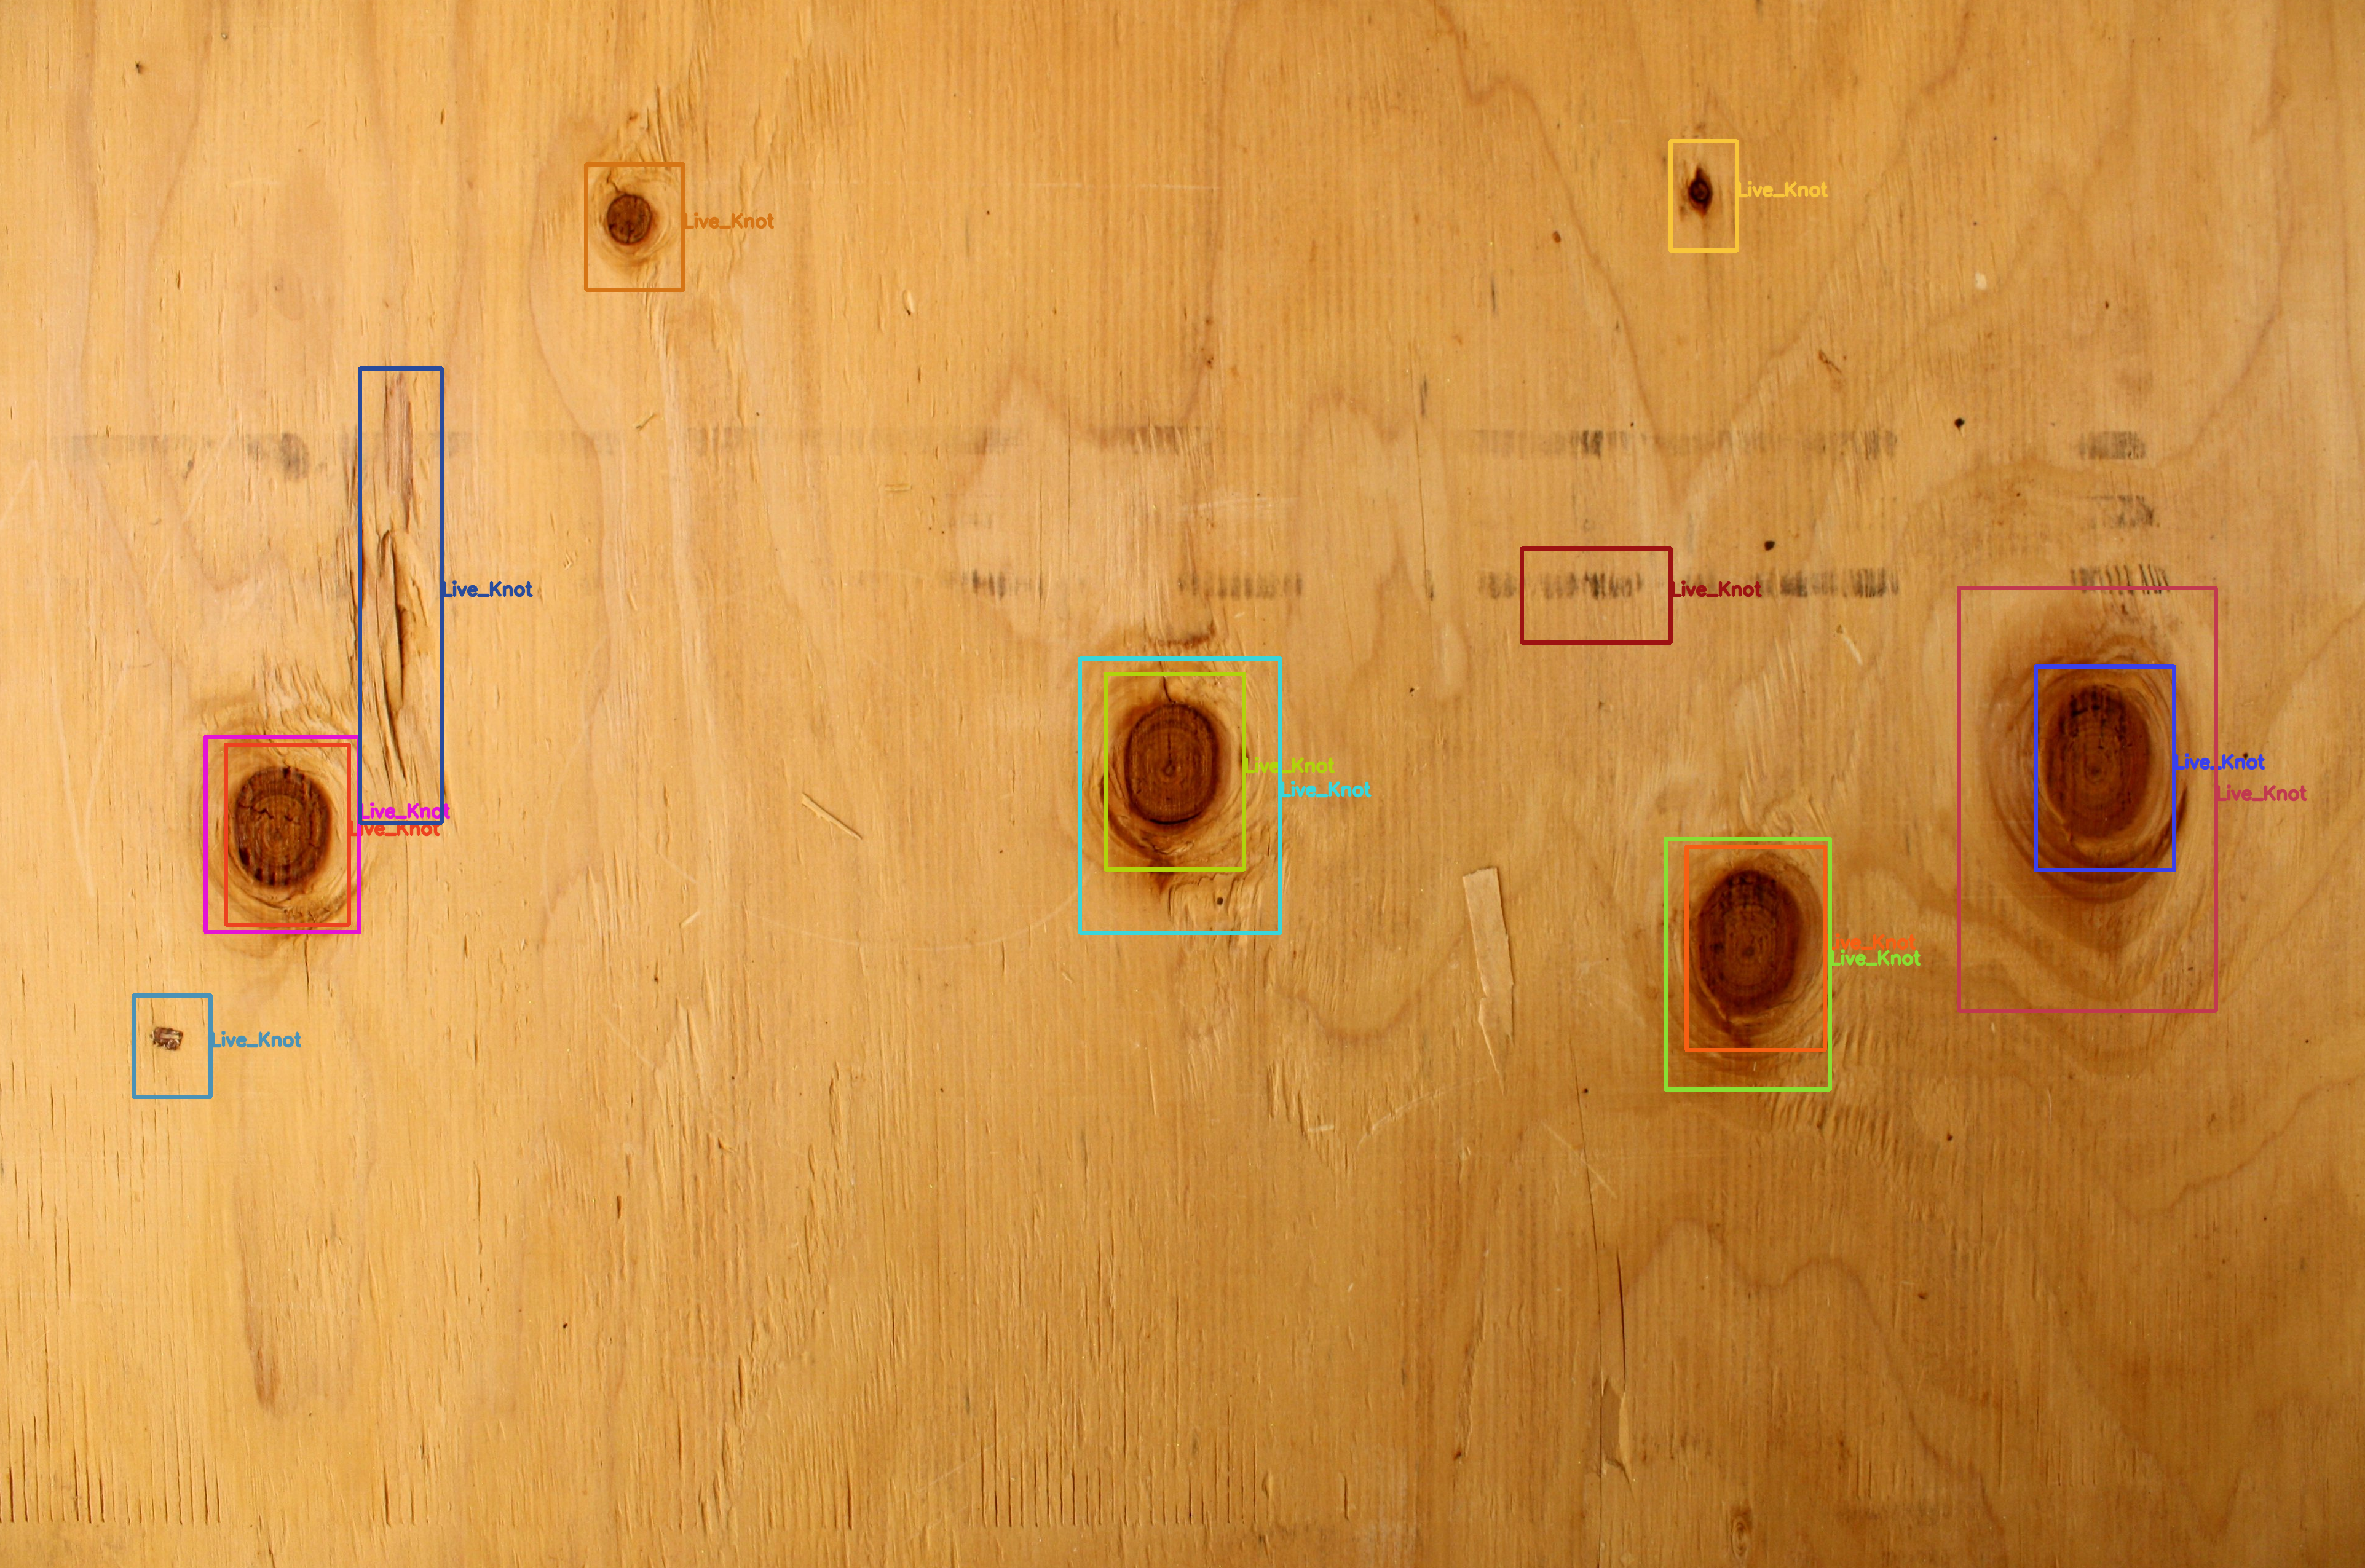
\includegraphics[width=0.4\textwidth]{3}}
			\caption{Метод оберненої матриці (а), метод Крамера (б), файл даних (в)}
		\end{figure}
		
		\section*{Висновок}
		На лабораторній роботі я засвоїв практичні навички використання методу оберненої матриці та методу Крамера та розробив функції для розв’язку системи лінійних алгебраїчних рівнянь 
		\begin{gather}\nonumber
			\left\{\begin{array}{@{}l@{}}
				0.34x_1 + 0.71x_2 + 0.63x_3 = 2.08\\\nonumber
				0.71x_1 - 0.65x_2 - 0.18x_3 = 0.17\\\nonumber
				1.17x_1 - 2.35x_2 + 0.75x_3 = 1.28\nonumber
			\end{array}\right.\,
		\end{gather}
		 за допомогою цих методів. Корені системи рівнянь: $-1.1786; -0.7041; 4.1915$.

	\end{large}
\end{document}
